
\section*{Potenz und Taylor Reihen}

\begin{tabular}{|c|c|c|c|}
\hline 
Taylor Koeffizient & Taylor Reihe & Konvergenzradius & Taylor Glied\tabularnewline
\hline 
\hline 
$a_{k}=\frac{f^{(k)}(x_{0})}{k!}$, $k=0,1,...$ & $t_{f}(x)=\sum_{k=0}^{inf}\frac{f^{(k)}(x_{0})}{k!}(x-x_{0})^{k}$ & $\rho=lim_{k\rightarrow\infty}|\frac{a_{k}}{a_{k+1}}|=lim_{k\rightarrow\infty}\frac{1}{\sqrt[k]{|a_{k}|}}$ & $\frac{f^{(k)}(x_{0})}{k!}(x-x_{0})^{k}$\tabularnewline
\hline 
\end{tabular}
\begin{itemize}
\item Innerhalb des Konvergenzradius darf:

\begin{itemize}
\item gliedweise abgeleitet werden
\item gliedweise integriert werden
\item gliedweise addiert, subtrahiert und multipliziert werden
\end{itemize}
\item Fehlerabschätzung

\begin{itemize}
\item alternierender Fall: $Fehler\leq|1.\, weggelassenes\, Glied|$
\item normaler Fall: $TaylorReihe(k\, Stelle)+Fehler\geq effektiver\, Wert$ 
\end{itemize}
\end{itemize}

\subsubsection*{Beispiele Taylorreihen}

\begin{tabular}{|l|l|l|l|}
\hline 
$arcsin(x),|x|<1$ & 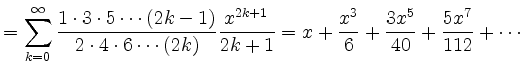
\includegraphics[height=1cm]{potenzreihen/img18} & $cos(x),x\in R$ & 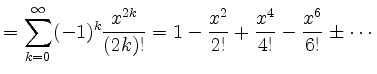
\includegraphics[height=1cm]{potenzreihen/img13}\tabularnewline
\hline 
$tan(x),|x|<\frac{\pi}{2}$ & 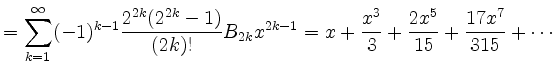
\includegraphics[height=1cm]{potenzreihen/img15} & $ln(1+x),-1<x\leq1$ & 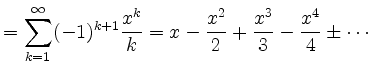
\includegraphics[height=1cm]{potenzreihen/img8}\tabularnewline
\hline 
$(1+x)^{a},|x|<1$ & 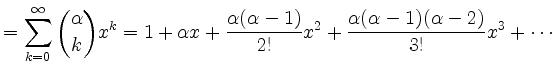
\includegraphics[height=1cm]{potenzreihen/img2} & $e^{x},x\in R$ & 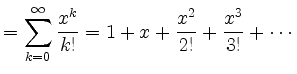
\includegraphics[height=1cm]{potenzreihen/img5}\tabularnewline
\hline 
$sin(x),x\in R$ & 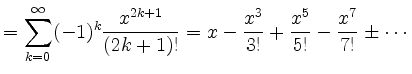
\includegraphics[height=1cm]{potenzreihen/img11} & $arctan(x),|x|<1$ & 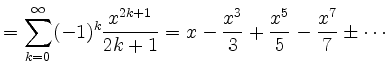
\includegraphics[height=1cm]{potenzreihen/img22}\tabularnewline
\hline 
$arccos(x),|x|<1^ {}$ & \multicolumn{2}{l|}{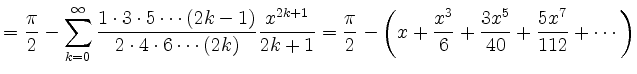
\includegraphics[height=1cm]{potenzreihen/img20}} & \tabularnewline
\hline 
\end{tabular}


\subsubsection*{Beispiel Herleitung Taylorreihe}

$f(x)=ln(x)\: bei\: x_{0}=1$

\begin{tabular}{|c|c|c|c|c|c|c|}
\cline{1-4} \cline{6-7} 
Ableitung & Koeffizient & Formel & Glied &  & \multicolumn{2}{c|}{Fakultäten}\tabularnewline
\cline{1-4} \cline{6-7} 
$f=ln(x)$  & $a_{0}=0$ & $\frac{f(1)}{0!}(x-1)^{0}$ & 0 & \multirow{6}{*}{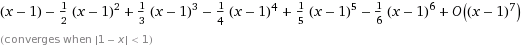
\includegraphics[height=1cm]{potenzreihen/wolfr1}} & 0! = 1 & 6! = 720\tabularnewline
\cline{1-4} \cline{6-7} 
$f'=\frac{1}{x}$ & $a_{1}=1$ & $\frac{f'(1)}{1!}(x-1)^{1}$ & $1(x-1)$ &  & 1! = 1 & 7! = 5040\tabularnewline
\cline{1-4} \cline{6-7} 
$f''=\frac{-1}{x^{2}}$ & $a_{2}=\frac{-1}{2}$ & $\frac{f''(1)}{2!}(x-1)^{2}$ & $\frac{-1}{2}(x-1)^{2}$ &  & 2! = 2 & 8! = 40320\tabularnewline
\cline{1-4} \cline{6-7} 
$f'''=\frac{2}{x^{3}}$ & $a_{3}=\frac{1}{3}$ & $\frac{f'''(1)}{3!}(x-1)^{3}$ & $\frac{1}{3}(x-1)^{3}$ &  & 3! = 6 & \tabularnewline
\cline{1-4} \cline{6-7} 
$f''''=-\frac{6}{x^{4}}$ & $a_{4}=\frac{-1}{4}$ & $\frac{f''''(1)}{4!}(x-1)^{4}$ & $\frac{-1}{4}(x-1)^{4}$ &  & 4! = 24 & \tabularnewline
\cline{1-4} \cline{6-7} 
 &  & $\frac{f^{(k)}(x_{0})}{k!}(x-x_{0})^{k}$ &  &  & 5! = 120 & \tabularnewline
\cline{1-4} \cline{6-7} 
\end{tabular}
